\subsection{Automatic differentiation}

Automatic differentiation (\textit{AD}) has a long and rich history, where its driving motivation is to efficiently calculate the derivatives of functions in a manner that is both correct and fast\cite{Baydin2015AutomaticDI}.
There are several different methods of implementing AD algorithms, such as source-code transformations or operator overloading.
These algorithms usually transform any program which implements some function to one that calculates its derivative.

There are two main variants of AD, namely forward-mode and reverse-mode AD.
In forward-mode AD, every term in the function trace is annotated with the corresponding derivative of that term.
These are also known as the respectively the primal and tangent traces.
So calculating the partial derivatives of sub-terms is structure preserving with respect to the normal calculation of terms.

This approach to forward-mode AD can be explained by dual numbers as these are, mathematically seen, what we are calculating with\cite{Baydin2015AutomaticDI}. Dual numbers are numbers of the form of
$$
  x + x' \epsilon
$$
where $x, x' \in \denR$ and $\epsilon$ is a nilpotent number, such that $\epsilon^2 = 0$ and $\epsilon \neq 0$.
Notably, both primal and tangent values are tracked in this representation, namely the tangent value is present in the coefficients of $\epsilon$.
As an example, we can see that this is true for both addition and multiplication:
\begin{align*}
  (x + x' \epsilon) + (y + y' \epsilon) &= (x + y) + (x' + y')\epsilon \\
  (x + x' \epsilon)(y + y' \epsilon) &= (xy) + (xy' + yx')\epsilon
\end{align*}
Using the following scheme for function application:
\begin{align*}
  f(x + x' \epsilon) &= f(x) + f'(x)x'\epsilon
\end{align*}
We can also see that it follows the chain rule for function composition.
\begin{align*}
  f(g(x + x' \epsilon)) &= f(g(x) + g'(x)x'\epsilon)) \\
    &= f(g(x)) + f'(g(x))g'(x)x'\epsilon
\end{align*}
Using this, we can essentially calculate the derivative of any derivable function by interpreting the non-dual number input $x$ as its dual number counterpart of $x + 0\epsilon$.

To give a more elaborate example of how this works in forward-mode AD, take the function $f(x, y) = x^2 + (x - y)$ as an example.
The dependencies between the terms and operations of the function is visible in the computational graph in Figure~\ref{fig:func_trace}.
The corresponding traces are filled in Table~\ref{table:func_trace} for the input values $x = 2, y = 1$.
We can calculate the partial derivative $\frac{\delta f}{\delta x}$ at this point by setting $x' = 1$ and $y' = 0$.
In this paper we will prove the correctness of a simple forward-mode automatic differentiation algorithm with respect to the semantics of a simply-typed lambda calculus.

Reverse-mode automatic differentiation takes a different approach.
It works backwards from the output by annotating each intermediate variable $v_i$ with an adjoint $v'_i=\frac{\delta y_i}{\delta v_i}$.
To do this, two passes are necessary.
Like the forward-mode variant, a primal trace is needed to determine the intermediate variables and their dependencies.
The second pass calculates the derivatives by working backwards from the output using the adjoints, also called the adjoint trace.

The optimal choice between automatic differentiation variant is heavily dependent on the specific function being differentiated.
Preference is given for forward-mode AD when the number of output variables exceeds the number of input variables, as it has to be rerun for each partial derivative of the function.
On the other hand, as reverse-mode AD works backwards, the reverse-pass needs to be redone for each output variable.
In machine learning research, reverse-mode AD is generally preferred as the objective functions generally contain a small number of output variables.

% TODO: Mention something about Eliott's categorical approach and its possible extension to a macro on combinators.

\begin{figure}
  \centering
  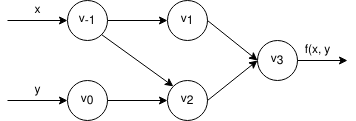
\includegraphics[scale=0.6]{./assets/function_trace.png}
  \caption{Computational graph of $f(x, y) = x^2 + (x - y)$}
  \label{fig:func_trace}
\end{figure}

\begin{table}
  \begin{center}
    \begin{tabular}{ l l l l l | l l l l l }
      \hline
      \multicolumn{5}{l}{Primal trace} & \multicolumn{5}{l}{Tangent trace} \\
      \hline
$v_{-1} $&$=$&$x$&$=$&$2$             &$v'_{-1}$&$=$&$x'$&$=$&$1$ \\
$v_0    $&$=$&$y$&$=$&$1$             &$v'_{0}$&$=$&$y'$&$=$&$0$ \\
      \hline
$v_1    $&$=$&$v_{-1}^2$&$=$&$4$      &$v'_{1}$&$=$&$2*v_{-1}$&$=$&$4$ \\
$v_2    $&$=$&$v_{-1} - v_{0}$&$=$&$1$&$v'_{2}$&$=$&$v'_{-1}-v'_{0}$&$=$&$1$ \\
$v_3    $&$=$&$v_1 + v_2$&$=$&$5$     &$v'_{3}$&$=$&$v'_1 + v'_2$&$=$&$5$ \\
      \hline
$f      $&$=$&$v_3$&$=$&$5$           &$f'$&$=$&$v'_3$&$=$&$5$ \\
      \hline
    \end{tabular}
  \end{center}
  \caption{Primal and tangent traces of $f(x, y) = x^2 + (x - y)$}
  \label{table:func_trace}
\end{table}
